\documentclass{beamer}

\usetheme{CambridgeUS}
\usecolortheme{dolphin}

\usepackage{wrapfig}
\usepackage{siunitx}
\usepackage{inconsolata}
\usepackage{amsmath}
\usepackage{bm}
\usepackage{adjustbox}
\usepackage{nicefrac}
\usepackage{listings}

\usepackage[backend=bibtex,style=authoryear]{biblatex}
\bibliography{common/references}
\AtBeginBibliography{\scriptsize}

% Tikz
\usepackage{tikz}
\usetikzlibrary{positioning,shapes,arrows,calc,intersections}
\usepackage{pgfplots}
\usepgfplotslibrary{dateplot}
\pgfplotsset{compat=1.8}

\DeclareMathOperator{\spann}{span}

\AtBeginSection[]{
  \begin{frame}
  \vfill
  \centering
  \begin{beamercolorbox}[sep=8pt,center,shadow=true,rounded=true]{title}
    \usebeamerfont{title}\insertsectionhead\par%
  \end{beamercolorbox}
  \vfill
  \end{frame}
}

\begin{document}

\title[Modern web infrastructure]{
  Modern web infrastructure: problems and solutions
}

\author[E.~Fonn]{E.~Fonn, K.~Johannessen}

\date[Mar 18, 2019]{March 18, 2019}

\titlegraphic{
  \includegraphics[height=0.05\textheight]{common/sintef} %\hspace{0.1\textheight}
}

\begin{frame}
  \titlepage
\end{frame}

\definecolor{darkblue}{HTML}{00688B}
\definecolor{darkgreen}{HTML}{6E8B3D}
\definecolor{cadet}{HTML}{DAE1FF}
\definecolor{salmon}{HTML}{FFB08A}

\tikzstyle{comp}=[
    draw=darkblue,
    fill=cadet,
    rounded corners=0.5mm,
    inner sep=2mm,
    text width=4cm,
    text centered,
]

\tikzstyle{file}=[
    draw=darkblue,
    fill=salmon,
    rounded corners=0.5mm,
    minimum height=6mm,
    inner sep=1mm,
]

\tikzstyle{src}=[
    draw=darkblue,
    fill=salmon!50,
    rounded corners=0.5mm,
    minimum height=6mm,
    inner sep=1mm,
]

\tikzstyle{brw}=[
    draw=darkblue,
    fill=cadet!20,
    minimum height=40mm,
    minimum width=40mm,
    rounded corners=0.5mm,
]

\tikzstyle{brwc}=[
    draw=darkblue,
    fill=salmon,
    rounded corners=2.6mm,
    inner sep=1.2mm,
    text width=12mm,
    text centered,
]

\tikzstyle{hidden}=[
    draw=black!0,
    fill=black!0,
    text=black!0,
]

% \begin{frame}
%   \begin{center}
%     \begin{tikzpicture}
%       \draw[dashed, black!30, very thick] (0,10) -- (0,0);

%       \node[file] (js) at (1,8) {JS};
%       \node[src, anchor=south] (ts) at ([yshift=2mm] js.north) {\scriptsize TS};
%       \node[file, anchor=west] (css) at ([xshift=2mm] js.east) {CSS};
%       \node[src, anchor=south] (scss) at ([yshift=2mm] css.north) {\scriptsize SCSS};
%       \node[file, anchor=west] (pics) at ([xshift=2mm] css.east) {Images};
%       \node[file, anchor=west] (fonts) at ([xshift=2mm] pics.east) {Fonts};
%       \node[file, anchor=west] (html) at ([xshift=2mm] fonts.east) {djHTML};
%       \draw[thick] ([yshift=-5mm] js.west) -- ([yshift=-5mm] html.east) node[midway, below] (disk) {Disk};

%       \node[comp] (nginx) at ([yshift=-12mm] disk) {Nginx};
%       \node[comp] (django) at ([yshift=-12mm] nginx) {Django};
%       \node[comp] (sql) at ([yshift=-12mm] django) {PostgreSQL};

%       \node[brw] (browser) at ([xshift=-43mm] nginx.west) {};
%       \node[brwc] (bhtml) at ([shift=(90:10mm)] browser) {HTML};
%       \node[brwc] (bcss) at ([shift=(210:10mm)] browser) {CSS};
%       \node[brwc] (bjs) at ([shift=(330:10mm)] browser) {JS};

%       \draw[<->] ([xshift=-1mm] bjs.north) -- ([xshift=2mm] bhtml.south);
%       \draw[<->] ([xshift=1mm] bcss.north) -- ([xshift=-2mm] bhtml.south);
%       \draw[<->] (bcss.east) -- (bjs.west);
%       \draw[->] (ts.south) -- (js.north);
%       \draw[->] (scss.south) -- (css.north);
%       \draw[<->] (disk.south) -- (nginx.north);
%       \draw[<->] (nginx.south) -- (django.north);
%       \draw[<->] (django.south) -- (sql.north);

%       \draw[<->] (browser.east) -- (nginx.west);
%       \draw (bjs.east) edge[out=0, in=180] ([yshift=-1mm] nginx.west);
%       \draw[<-] (bjs.east) -- ([xshift=0.1mm] bjs.east);
%       \draw[->] ([xshift=-0.1mm, yshift=-1mm] nginx.west) -- ([yshift=-1mm] nginx.west);
%       \draw[<->] (django.east) -| ([xshift=2mm] html.south);
%     \end{tikzpicture}
%   \end{center}
% \end{frame}

\begin{frame}
  \frametitle{1: How to communicate over the internet?}

  \begin{itemize}
  \item HTTP: Hyper-Text Transfer Protocol
  \item Defines the ``legal'' form of a request and a response
  \item Two type of requests: GET and POST
  \item Many types of response (you have probably seen some of these)
    \begin{itemize}
    \item 200: OK
    \item 403: Forbidden
    \item 404: Not found
    \item 500: Internal server error
    \item 503: Service unavailable
    \item 418: I'm a teapot
    \item etc.
    \end{itemize}
  \end{itemize}
\end{frame}

\begin{frame}
  \begin{center}
    \begin{tikzpicture}
      \draw[dashed, black!30, very thick] (0,10) -- (0,0);

      \node[file, hidden] (js) at (1,8) {JS};
      \node[src, hidden, anchor=south] (ts) at ([yshift=2mm] js.north) {\scriptsize TS};
      \node[file, hidden, anchor=west] (css) at ([xshift=2mm] js.east) {CSS};
      \node[src, hidden, anchor=south] (scss) at ([yshift=2mm] css.north) {\scriptsize SCSS};
      \node[file, hidden, anchor=west] (pics) at ([xshift=2mm] css.east) {Images};
      \node[file, hidden, anchor=west] (fonts) at ([xshift=2mm] pics.east) {Fonts};
      \node[file, hidden, anchor=west] (html) at ([xshift=2mm] fonts.east) {djHTML};
      \draw[thick, hidden] ([yshift=-5mm] js.west) -- ([yshift=-5mm] html.east) node[midway, below] (disk) {Disk};

      \node[comp, hidden] (nginx) at ([yshift=-12mm] disk) {Nginx};
      \node[comp, hidden] (django) at ([yshift=-12mm] nginx) {Django};
      \node[comp, hidden] (sql) at ([yshift=-12mm] django) {PostgreSQL};

      \node[brw, hidden] (browser) at ([xshift=-43mm] nginx.west) {};
      \node[brwc, hidden] (bhtml) at ([shift=(90:10mm)] browser) {HTML};
      \node[brwc, hidden] (bcss) at ([shift=(210:10mm)] browser) {CSS};
      \node[brwc, hidden] (bjs) at ([shift=(330:10mm)] browser) {JS};

      \draw[<->, hidden] ([xshift=-1mm] bjs.north) -- ([xshift=2mm] bhtml.south);
      \draw[<->, hidden] ([xshift=1mm] bcss.north) -- ([xshift=-2mm] bhtml.south);
      \draw[<->, hidden] (bcss.east) -- (bjs.west);
      \draw[->, hidden] (ts.south) -- (js.north);
      \draw[->, hidden] (scss.south) -- (css.north);
      \draw[<->, hidden] (disk.south) -- (nginx.north);
      \draw[<->, hidden] (nginx.south) -- (django.north);
      \draw[<->, hidden] (django.south) -- (sql.north);

      \draw[<->] (browser.east) -- (nginx.west);
      \draw[hidden] (bjs.east) edge[out=0, in=180] ([yshift=-1mm] nginx.west);
      \draw[<-, hidden] (bjs.east) -- ([xshift=0.1mm] bjs.east);
      \draw[->, hidden] ([xshift=-0.1mm, yshift=-1mm] nginx.west) -- ([yshift=-1mm] nginx.west);
      \draw[<->, hidden] (django.east) -| ([xshift=2mm] html.south);
    \end{tikzpicture}
  \end{center}
\end{frame}

\begin{frame}[fragile]
  \frametitle{2: How to respond with a meaningful webpage?}

  \begin{itemize}
  \item HTML: Hyper-Text Markup Language
  \item Typically contains text, paragraphs, logical structure and
    references to other resources.
  \item HTML is what makes the ``web'' different from the
    ``internet''.
  \end{itemize}

  \begin{lstlisting}[basicstyle=\ttfamily]
<h1>Welcome to my website</h1>
<p>Text in a paragraph.</p>
<a href="http://sintef.no">Good science here</a>
<strong>Bold</strong>, <em>italic</em>, etc.
  \end{lstlisting}
\end{frame}

\begin{frame}
  \begin{center}
    \begin{tikzpicture}
      \draw[dashed, black!30, very thick] (0,10) -- (0,0);

      \node[file, hidden] (js) at (1,8) {JS};
      \node[src, hidden, anchor=south] (ts) at ([yshift=2mm] js.north) {\scriptsize TS};
      \node[file, hidden, anchor=west] (css) at ([xshift=2mm] js.east) {CSS};
      \node[src, hidden, anchor=south] (scss) at ([yshift=2mm] css.north) {\scriptsize SCSS};
      \node[file, hidden, anchor=west] (pics) at ([xshift=2mm] css.east) {Images};
      \node[file, hidden, anchor=west] (fonts) at ([xshift=2mm] pics.east) {Fonts};
      \node[file, anchor=west] (html) at ([xshift=2mm] fonts.east) {HTML};
      \draw[thick] ([yshift=-5mm] js.west) -- ([yshift=-5mm] html.east) node[midway, below] (disk) {Disk};

      \node[comp] (nginx) at ([yshift=-12mm] disk) {Nginx};
      \node[comp, hidden] (django) at ([yshift=-12mm] nginx) {Django};
      \node[comp, hidden] (sql) at ([yshift=-12mm] django) {PostgreSQL};

      \node[brw, hidden] (browser) at ([xshift=-43mm] nginx.west) {};
      \node[brwc, hidden] (bhtml) at ([shift=(90:10mm)] browser) {HTML};
      \node[brwc, hidden] (bcss) at ([shift=(210:10mm)] browser) {CSS};
      \node[brwc, hidden] (bjs) at ([shift=(330:10mm)] browser) {JS};

      \draw[<->, hidden] ([xshift=-1mm] bjs.north) -- ([xshift=2mm] bhtml.south);
      \draw[<->, hidden] ([xshift=1mm] bcss.north) -- ([xshift=-2mm] bhtml.south);
      \draw[<->, hidden] (bcss.east) -- (bjs.west);
      \draw[->, hidden] (ts.south) -- (js.north);
      \draw[->, hidden] (scss.south) -- (css.north);
      \draw[<->] (disk.south) -- (nginx.north);
      \draw[<->, hidden] (nginx.south) -- (django.north);
      \draw[<->, hidden] (django.south) -- (sql.north);

      \draw[<->] (browser.east) -- (nginx.west);
      \draw[hidden] (bjs.east) edge[out=0, in=180] ([yshift=-1mm] nginx.west);
      \draw[<-, hidden] (bjs.east) -- ([xshift=0.1mm] bjs.east);
      \draw[->, hidden] ([xshift=-0.1mm, yshift=-1mm] nginx.west) -- ([yshift=-1mm] nginx.west);
      % \draw[<->, hidden] (django.east) -| ([xshift=2mm] html.south);
    \end{tikzpicture}
  \end{center}
\end{frame}

\begin{frame}
  \frametitle{3: How to show a webpage?}

  \begin{itemize}
  \item The first \emph{web browser} was Netscape Navigator, released
    in 1994.
  \item Since HTML was relatively loosely defined, browsers had to be
    very generous and accept a lot of variety.
  \end{itemize}

  \begin{center}
    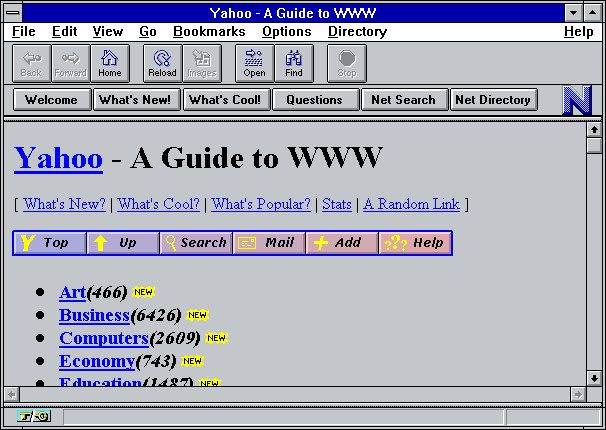
\includegraphics[height=0.5\textheight]{netscape}
  \end{center}
\end{frame}

\begin{frame}
  \begin{center}
    \begin{tikzpicture}
      \draw[dashed, black!30, very thick] (0,10) -- (0,0);

      \node[file, hidden] (js) at (1,8) {JS};
      \node[src, hidden, anchor=south] (ts) at ([yshift=2mm] js.north) {\scriptsize TS};
      \node[file, hidden, anchor=west] (css) at ([xshift=2mm] js.east) {CSS};
      \node[src, hidden, anchor=south] (scss) at ([yshift=2mm] css.north) {\scriptsize SCSS};
      \node[file, hidden, anchor=west] (pics) at ([xshift=2mm] css.east) {Images};
      \node[file, hidden, anchor=west] (fonts) at ([xshift=2mm] pics.east) {Fonts};
      \node[file, anchor=west] (html) at ([xshift=2mm] fonts.east) {HTML};
      \draw[thick] ([yshift=-5mm] js.west) -- ([yshift=-5mm] html.east) node[midway, below] (disk) {Disk};

      \node[comp] (nginx) at ([yshift=-12mm] disk) {Nginx};
      \node[comp, hidden] (django) at ([yshift=-12mm] nginx) {Django};
      \node[comp, hidden] (sql) at ([yshift=-12mm] django) {PostgreSQL};

      \node[brw] (browser) at ([xshift=-43mm] nginx.west) {};
      \node[brwc] (bhtml) at ([shift=(90:10mm)] browser) {HTML};
      % \node[brwc, hidden] (bcss) at ([shift=(210:10mm)] browser) {CSS};
      % \node[brwc, hidden] (bjs) at ([shift=(330:10mm)] browser) {JS};

      % \draw[<->, hidden] ([xshift=-1mm] bjs.north) -- ([xshift=2mm] bhtml.south);
      % \draw[<->, hidden] ([xshift=1mm] bcss.north) -- ([xshift=-2mm] bhtml.south);
      % \draw[<->, hidden] (bcss.east) -- (bjs.west);
      \draw[->, hidden] (ts.south) -- (js.north);
      \draw[->, hidden] (scss.south) -- (css.north);
      \draw[<->] (disk.south) -- (nginx.north);
      \draw[<->, hidden] (nginx.south) -- (django.north);
      \draw[<->, hidden] (django.south) -- (sql.north);

      \draw[<->] (browser.east) -- (nginx.west);
      % \draw[hidden] (bjs.east) edge[out=0, in=180] ([yshift=-1mm] nginx.west);
      \draw[<-, hidden] (bjs.east) -- ([xshift=0.1mm] bjs.east);
      \draw[->, hidden] ([xshift=-0.1mm, yshift=-1mm] nginx.west) -- ([yshift=-1mm] nginx.west);
      % \draw[<->, hidden] (django.east) -| ([xshift=2mm] html.south);
    \end{tikzpicture}
  \end{center}
\end{frame}

\begin{frame}[fragile]
  \frametitle{4: How to serve dynamic content?}

  \begin{itemize}
  \item Instead of a static server like Nginx, use a server
    that can generate HTML on the fly, like \emph{Django}.
  \item Django is actually a framework for writing your own server, a
    sort of get-started kit.
  \item Instead of HTML, we have a \emph{templating language} called
    djHTML.
  \end{itemize}

  \begin{lstlisting}[basicstyle=\ttfamily]
<h1>{{ title|titlecase }}</h1>
<p>Text in a paragraph.</p>

<a href="{{ target_address }}">Good science here</a>

<strong>Bold</strong>, <em>italic</em>, etc.
  \end{lstlisting}
\end{frame}

\begin{frame}
  \begin{center}
    \begin{tikzpicture}
      \draw[dashed, black!30, very thick] (0,10) -- (0,0);

      \node[file, hidden] (js) at (1,8) {JS};
      \node[src, hidden, anchor=south] (ts) at ([yshift=2mm] js.north) {\scriptsize TS};
      \node[file, hidden, anchor=west] (css) at ([xshift=2mm] js.east) {CSS};
      \node[src, hidden, anchor=south] (scss) at ([yshift=2mm] css.north) {\scriptsize SCSS};
      \node[file, hidden, anchor=west] (pics) at ([xshift=2mm] css.east) {Images};
      \node[file, hidden, anchor=west] (fonts) at ([xshift=2mm] pics.east) {Fonts};
      \node[file, anchor=west] (html) at ([xshift=2mm] fonts.east) {djHTML};
      \draw[thick] ([yshift=-5mm] js.west) -- ([yshift=-5mm] html.east) node[midway, below] (disk) {Disk};

      \node[comp] (nginx) at ([yshift=-12mm] disk) {Django};
      \node[comp, hidden] (django) at ([yshift=-12mm] nginx) {Django};
      \node[comp, hidden] (sql) at ([yshift=-12mm] django) {PostgreSQL};

      \node[brw] (browser) at ([xshift=-43mm] nginx.west) {};
      \node[brwc] (bhtml) at ([shift=(90:10mm)] browser) {HTML};
      % \node[brwc, hidden] (bcss) at ([shift=(210:10mm)] browser) {CSS};
      % \node[brwc, hidden] (bjs) at ([shift=(330:10mm)] browser) {JS};

      % \draw[<->, hidden] ([xshift=-1mm] bjs.north) -- ([xshift=2mm] bhtml.south);
      % \draw[<->, hidden] ([xshift=1mm] bcss.north) -- ([xshift=-2mm] bhtml.south);
      % \draw[<->, hidden] (bcss.east) -- (bjs.west);
      \draw[->, hidden] (ts.south) -- (js.north);
      \draw[->, hidden] (scss.south) -- (css.north);
      \draw[<->] (disk.south) -- (nginx.north);
      \draw[<->, hidden] (nginx.south) -- (django.north);
      \draw[<->, hidden] (django.south) -- (sql.north);

      \draw[<->] (browser.east) -- (nginx.west);
      % \draw[hidden] (bjs.east) edge[out=0, in=180] ([yshift=-1mm] nginx.west);
      \draw[<-, hidden] (bjs.east) -- ([xshift=0.1mm] bjs.east);
      \draw[->, hidden] ([xshift=-0.1mm, yshift=-1mm] nginx.west) -- ([yshift=-1mm] nginx.west);
      % \draw[<->, hidden] (django.east) -| ([xshift=2mm] html.south);
    \end{tikzpicture}
  \end{center}
\end{frame}

\begin{frame}
  \frametitle{5: How to remember information?}

  \begin{itemize}
  \item After responding to a request, the server immediately forgets
    all about it.
  \item Data is typically stored in a relational database, like
    PostgreSQL.
  \item This database is not visible from outside and can only be
    interacted with by the server.
  \item Django has special functionality for interacting with
    databases.
  \end{itemize}
\end{frame}

\begin{frame}
  \begin{center}
    \begin{tikzpicture}
      \draw[dashed, black!30, very thick] (0,10) -- (0,0);

      \node[file, hidden] (js) at (1,8) {JS};
      \node[src, hidden, anchor=south] (ts) at ([yshift=2mm] js.north) {\scriptsize TS};
      \node[file, hidden, anchor=west] (css) at ([xshift=2mm] js.east) {CSS};
      \node[src, hidden, anchor=south] (scss) at ([yshift=2mm] css.north) {\scriptsize SCSS};
      \node[file, hidden, anchor=west] (pics) at ([xshift=2mm] css.east) {Images};
      \node[file, hidden, anchor=west] (fonts) at ([xshift=2mm] pics.east) {Fonts};
      \node[file, anchor=west] (html) at ([xshift=2mm] fonts.east) {djHTML};
      \draw[thick] ([yshift=-5mm] js.west) -- ([yshift=-5mm] html.east) node[midway, below] (disk) {Disk};

      \node[comp] (nginx) at ([yshift=-12mm] disk) {Django};
      \node[comp] (django) at ([yshift=-12mm] nginx) {PostgreSQL};
      \node[comp, hidden] (sql) at ([yshift=-12mm] django) {PostgreSQL};

      \node[brw] (browser) at ([xshift=-43mm] nginx.west) {};
      \node[brwc] (bhtml) at ([shift=(90:10mm)] browser) {HTML};
      % \node[brwc, hidden] (bcss) at ([shift=(210:10mm)] browser) {CSS};
      % \node[brwc, hidden] (bjs) at ([shift=(330:10mm)] browser) {JS};

      % \draw[<->, hidden] ([xshift=-1mm] bjs.north) -- ([xshift=2mm] bhtml.south);
      % \draw[<->, hidden] ([xshift=1mm] bcss.north) -- ([xshift=-2mm] bhtml.south);
      % \draw[<->, hidden] (bcss.east) -- (bjs.west);
      \draw[->, hidden] (ts.south) -- (js.north);
      \draw[->, hidden] (scss.south) -- (css.north);
      \draw[<->] (disk.south) -- (nginx.north);
      \draw[<->] (nginx.south) -- (django.north);
      \draw[<->, hidden] (django.south) -- (sql.north);

      \draw[<->] (browser.east) -- (nginx.west);
      % \draw[hidden] (bjs.east) edge[out=0, in=180] ([yshift=-1mm] nginx.west);
      \draw[<-, hidden] (bjs.east) -- ([xshift=0.1mm] bjs.east);
      \draw[->, hidden] ([xshift=-0.1mm, yshift=-1mm] nginx.west) -- ([yshift=-1mm] nginx.west);
      % \draw[<->, hidden] (django.east) -| ([xshift=2mm] html.south);
    \end{tikzpicture}
  \end{center}
\end{frame}

\begin{frame}
  \frametitle{6: How to remember temporary data?}

  \begin{itemize}
  \item It's (close to) impossible for the server to recognize that
    two consecutive requests come from the same user.
  \item Closely related problem: how to keep a user logged in without
    having to type a password on every single new request.
  \item \emph{Cookies} solve this problem: a small data package added
    to every request and every response.
  \item Django automatically handles authentication via cookies.
  \end{itemize}
\end{frame}

\begin{frame}
  \begin{center}
    \begin{tikzpicture}
      \draw[dashed, black!30, very thick] (0,10) -- (0,0);

      \node[file, hidden] (js) at (1,8) {JS};
      \node[src, hidden, anchor=south] (ts) at ([yshift=2mm] js.north) {\scriptsize TS};
      \node[file, hidden, anchor=west] (css) at ([xshift=2mm] js.east) {CSS};
      \node[src, hidden, anchor=south] (scss) at ([yshift=2mm] css.north) {\scriptsize SCSS};
      \node[file, hidden, anchor=west] (pics) at ([xshift=2mm] css.east) {Images};
      \node[file, hidden, anchor=west] (fonts) at ([xshift=2mm] pics.east) {Fonts};
      \node[file, anchor=west] (html) at ([xshift=2mm] fonts.east) {djHTML};
      \draw[thick] ([yshift=-5mm] js.west) -- ([yshift=-5mm] html.east) node[midway, below] (disk) {Disk};

      \node[comp] (nginx) at ([yshift=-12mm] disk) {Django};
      \node[comp] (django) at ([yshift=-12mm] nginx) {PostgreSQL};
      \node[comp, hidden] (sql) at ([yshift=-12mm] django) {PostgreSQL};

      \node[brw] (browser) at ([xshift=-43mm] nginx.west) {};
      \node[brwc] (bhtml) at ([shift=(90:10mm)] browser) {HTML};
      % \node[brwc, hidden] (bcss) at ([shift=(210:10mm)] browser) {CSS};
      % \node[brwc, hidden] (bjs) at ([shift=(330:10mm)] browser) {JS};

      % \draw[<->, hidden] ([xshift=-1mm] bjs.north) -- ([xshift=2mm] bhtml.south);
      % \draw[<->, hidden] ([xshift=1mm] bcss.north) -- ([xshift=-2mm] bhtml.south);
      % \draw[<->, hidden] (bcss.east) -- (bjs.west);
      \draw[->, hidden] (ts.south) -- (js.north);
      \draw[->, hidden] (scss.south) -- (css.north);
      \draw[<->] (disk.south) -- (nginx.north);
      \draw[<->] (nginx.south) -- (django.north);
      \draw[<->, hidden] (django.south) -- (sql.north);

      \draw[<->] (browser.east) -- (nginx.west) node[midway, above] {\scriptsize {\bf +}cookies};
      % \draw[hidden] (bjs.east) edge[out=0, in=180] ([yshift=-1mm] nginx.west);
      \draw[<-, hidden] (bjs.east) -- ([xshift=0.1mm] bjs.east);
      \draw[->, hidden] ([xshift=-0.1mm, yshift=-1mm] nginx.west) -- ([yshift=-1mm] nginx.west);
      % \draw[<->, hidden] (django.east) -| ([xshift=2mm] html.south);
    \end{tikzpicture}
  \end{center}
\end{frame}

\begin{frame}
  \frametitle{7: My website looks like it's 1994}

  \begin{itemize}
  \item HTML has very limited means for style.
  \item CSS: Cascading Style-Sheets was invented in 1996 to solve this problem.
  \item A stylesheet contains a list of \emph{rules} for how different
    HTML objects should look.
  \item It's normal for the HTML document to include a link to the CSS
    file, so that the browser makes a secondary request for it.
  \item Same goes for other artistic details like images, fonts, etc.
  \end{itemize}
\end{frame}

\begin{frame}
  \begin{center}
    \begin{tikzpicture}
      \draw[dashed, black!30, very thick] (0,10) -- (0,0);

      \node[file, hidden] (js) at (1,8) {JS};
      \node[src, hidden, anchor=south] (ts) at ([yshift=2mm] js.north) {\scriptsize TS};
      \node[file, anchor=west] (css) at ([xshift=2mm] js.east) {CSS};
      \node[src, hidden, anchor=south] (scss) at ([yshift=2mm] css.north) {\scriptsize SCSS};
      \node[file, anchor=west] (pics) at ([xshift=2mm] css.east) {Images};
      \node[file, anchor=west] (fonts) at ([xshift=2mm] pics.east) {Fonts};
      \node[file, anchor=west] (html) at ([xshift=2mm] fonts.east) {djHTML};
      \draw[thick] ([yshift=-5mm] js.west) -- ([yshift=-5mm] html.east) node[midway, below] (disk) {Disk};

      \node[comp] (nginx) at ([yshift=-12mm] disk) {Django};
      \node[comp] (django) at ([yshift=-12mm] nginx) {PostgreSQL};
      \node[comp, hidden] (sql) at ([yshift=-12mm] django) {PostgreSQL};

      \node[brw] (browser) at ([xshift=-43mm] nginx.west) {};
      \node[brwc] (bhtml) at ([shift=(90:10mm)] browser) {HTML};
      \node[brwc] (bcss) at ([shift=(210:10mm)] browser) {CSS};
      % \node[brwc, hidden] (bjs) at ([shift=(330:10mm)] browser) {JS};

      % \draw[<->, hidden] ([xshift=-1mm] bjs.north) -- ([xshift=2mm] bhtml.south);
      \draw[<->] ([xshift=1mm] bcss.north) -- ([xshift=-2mm] bhtml.south);
      % \draw[<->, hidden] (bcss.east) -- (bjs.west);
      \draw[->, hidden] (ts.south) -- (js.north);
      \draw[->, hidden] (scss.south) -- (css.north);
      \draw[<->] (disk.south) -- (nginx.north);
      \draw[<->] (nginx.south) -- (django.north);
      \draw[<->, hidden] (django.south) -- (sql.north);

      \draw[<->] (browser.east) -- (nginx.west) node[midway, above] {\scriptsize {\bf +}cookies};
      % \draw[hidden] (bjs.east) edge[out=0, in=180] ([yshift=-1mm] nginx.west);
      \draw[<-, hidden] (bjs.east) -- ([xshift=0.1mm] bjs.east);
      \draw[->, hidden] ([xshift=-0.1mm, yshift=-1mm] nginx.west) -- ([yshift=-1mm] nginx.west);
      % \draw[<->, hidden] (django.east) -| ([xshift=2mm] html.south);
    \end{tikzpicture}
  \end{center}
\end{frame}

\begin{frame}
  \frametitle{8: How to make my website \emph{do} things?}

  \begin{itemize}
  \item HTML is fully static. The only way to make ``things happen''
    is to make a new request to the server.
  \item Many forms of ``dynamism'' are better handled using
    Javascript, a programming language that can run \emph{in the
      browser} without making any new requests.
  \item Like CSS, JS is sent to the browser via a separate request.
  \end{itemize}
\end{frame}

\begin{frame}
  \begin{center}
    \begin{tikzpicture}
      \draw[dashed, black!30, very thick] (0,10) -- (0,0);

      \node[file] (js) at (1,8) {JS};
      \node[src, hidden, anchor=south] (ts) at ([yshift=2mm] js.north) {\scriptsize TS};
      \node[file, anchor=west] (css) at ([xshift=2mm] js.east) {CSS};
      \node[src, hidden, anchor=south] (scss) at ([yshift=2mm] css.north) {\scriptsize SCSS};
      \node[file, anchor=west] (pics) at ([xshift=2mm] css.east) {Images};
      \node[file, anchor=west] (fonts) at ([xshift=2mm] pics.east) {Fonts};
      \node[file, anchor=west] (html) at ([xshift=2mm] fonts.east) {djHTML};
      \draw[thick] ([yshift=-5mm] js.west) -- ([yshift=-5mm] html.east) node[midway, below] (disk) {Disk};

      \node[comp] (nginx) at ([yshift=-12mm] disk) {Django};
      \node[comp] (django) at ([yshift=-12mm] nginx) {PostgreSQL};
      \node[comp, hidden] (sql) at ([yshift=-12mm] django) {PostgreSQL};

      \node[brw] (browser) at ([xshift=-43mm] nginx.west) {};
      \node[brwc] (bhtml) at ([shift=(90:10mm)] browser) {HTML};
      \node[brwc] (bcss) at ([shift=(210:10mm)] browser) {CSS};
      \node[brwc] (bjs) at ([shift=(330:10mm)] browser) {JS};

      \draw[<->] ([xshift=-1mm] bjs.north) -- ([xshift=2mm] bhtml.south);
      \draw[<->] ([xshift=1mm] bcss.north) -- ([xshift=-2mm] bhtml.south);
      \draw[<->] (bcss.east) -- (bjs.west);
      \draw[->, hidden] (ts.south) -- (js.north);
      \draw[->, hidden] (scss.south) -- (css.north);
      \draw[<->] (disk.south) -- (nginx.north);
      \draw[<->] (nginx.south) -- (django.north);
      \draw[<->, hidden] (django.south) -- (sql.north);

      \draw[<->] (browser.east) -- (nginx.west) node[midway, above] {\scriptsize {\bf +}cookies};
      % \draw[hidden] (bjs.east) edge[out=0, in=180] ([yshift=-1mm] nginx.west);
      \draw[<-, hidden] (bjs.east) -- ([xshift=0.1mm] bjs.east);
      \draw[->, hidden] ([xshift=-0.1mm, yshift=-1mm] nginx.west) -- ([yshift=-1mm] nginx.west);
      % \draw[<->, hidden] (django.east) -| ([xshift=2mm] html.south);
    \end{tikzpicture}
  \end{center}
\end{frame}

\begin{frame}
  \frametitle{9: Now my website is really slow}

  \begin{itemize}
  \item Displaying a typical webpage now means at least one request
    for the HTML and several more for the JS, CSS, images and fonts to
    go with it.
  \item Web frameworks like Django are designed for features and not
    speed. Serving static content slows them down.
  \item Common: a multi-layered webserver design with a fast
    front-facing server for static content, which proxies the requests
    for dynamic content to a slower server in the back.
  \end{itemize}
\end{frame}

\begin{frame}
  \begin{center}
    \begin{tikzpicture}
      \draw[dashed, black!30, very thick] (0,10) -- (0,0);

      \node[file] (js) at (1,8) {JS};
      \node[src, hidden, anchor=south] (ts) at ([yshift=2mm] js.north) {\scriptsize TS};
      \node[file, anchor=west] (css) at ([xshift=2mm] js.east) {CSS};
      \node[src, hidden, anchor=south] (scss) at ([yshift=2mm] css.north) {\scriptsize SCSS};
      \node[file, anchor=west] (pics) at ([xshift=2mm] css.east) {Images};
      \node[file, anchor=west] (fonts) at ([xshift=2mm] pics.east) {Fonts};
      \node[file, anchor=west] (html) at ([xshift=2mm] fonts.east) {djHTML};
      \draw[thick] ([yshift=-5mm] js.west) -- ([yshift=-5mm] html.east) node[midway, below] (disk) {Disk};

      \node[comp] (nginx) at ([yshift=-12mm] disk) {Nginx};
      \node[comp] (django) at ([yshift=-12mm] nginx) {Django};
      \node[comp] (sql) at ([yshift=-12mm] django) {PostgreSQL};

      \node[brw] (browser) at ([xshift=-43mm] nginx.west) {};
      \node[brwc] (bhtml) at ([shift=(90:10mm)] browser) {HTML};
      \node[brwc] (bcss) at ([shift=(210:10mm)] browser) {CSS};
      \node[brwc] (bjs) at ([shift=(330:10mm)] browser) {JS};

      \draw[<->] ([xshift=-1mm] bjs.north) -- ([xshift=2mm] bhtml.south);
      \draw[<->] ([xshift=1mm] bcss.north) -- ([xshift=-2mm] bhtml.south);
      \draw[<->] (bcss.east) -- (bjs.west);
      \draw[->, hidden] (ts.south) -- (js.north);
      \draw[->, hidden] (scss.south) -- (css.north);
      \draw[<->] (disk.south) -- (nginx.north);
      \draw[<->] (nginx.south) -- (django.north);
      \draw[<->] (django.south) -- (sql.north);

      \draw[<->] (browser.east) -- (nginx.west) node[midway, above] {\scriptsize {\bf +}cookies};
      % \draw[hidden] (bjs.east) edge[out=0, in=180] ([yshift=-1mm] nginx.west);
      \draw[<-, hidden] (bjs.east) -- ([xshift=0.1mm] bjs.east);
      \draw[->, hidden] ([xshift=-0.1mm, yshift=-1mm] nginx.west) -- ([yshift=-1mm] nginx.west);
      \draw[<->] (django.east) -| ([xshift=2mm] html.south);
    \end{tikzpicture}
  \end{center}
\end{frame}

\begin{frame}
  \frametitle{10: HTML, CSS and JS are dinosaurs}

  \begin{itemize}
  \item These languages suffer from 20 years of baggage, having been
    originally designed for much more limited things than they are
    used for today.
  \item The languages are now standardized, but the wide array of user
    software still in use means that we can't rely too much on these
    standards.
  \item CSS and JS can be \emph{generated} by compiling other, more
    sensible languages: SASS (Syntactically Awesome Style-Sheets)
    generates CSS and TS (Typescript) generates JS.
  \end{itemize}
\end{frame}

\begin{frame}
  \begin{center}
    \begin{tikzpicture}
      \draw[dashed, black!30, very thick] (0,10) -- (0,0);

      \node[file] (js) at (1,8) {JS};
      \node[src, anchor=south] (ts) at ([yshift=2mm] js.north) {\scriptsize TS};
      \node[file, anchor=west] (css) at ([xshift=2mm] js.east) {CSS};
      \node[src, anchor=south] (scss) at ([yshift=2mm] css.north) {\scriptsize SCSS};
      \node[file, anchor=west] (pics) at ([xshift=2mm] css.east) {Images};
      \node[file, anchor=west] (fonts) at ([xshift=2mm] pics.east) {Fonts};
      \node[file, anchor=west] (html) at ([xshift=2mm] fonts.east) {djHTML};
      \draw[thick] ([yshift=-5mm] js.west) -- ([yshift=-5mm] html.east) node[midway, below] (disk) {Disk};

      \node[comp] (nginx) at ([yshift=-12mm] disk) {Nginx};
      \node[comp] (django) at ([yshift=-12mm] nginx) {Django};
      \node[comp] (sql) at ([yshift=-12mm] django) {PostgreSQL};

      \node[brw] (browser) at ([xshift=-43mm] nginx.west) {};
      \node[brwc] (bhtml) at ([shift=(90:10mm)] browser) {HTML};
      \node[brwc] (bcss) at ([shift=(210:10mm)] browser) {CSS};
      \node[brwc] (bjs) at ([shift=(330:10mm)] browser) {JS};

      \draw[<->] ([xshift=-1mm] bjs.north) -- ([xshift=2mm] bhtml.south);
      \draw[<->] ([xshift=1mm] bcss.north) -- ([xshift=-2mm] bhtml.south);
      \draw[<->] (bcss.east) -- (bjs.west);
      \draw[->] (ts.south) -- (js.north);
      \draw[->] (scss.south) -- (css.north);
      \draw[<->] (disk.south) -- (nginx.north);
      \draw[<->] (nginx.south) -- (django.north);
      \draw[<->] (django.south) -- (sql.north);

      \draw[<->] (browser.east) -- (nginx.west) node[midway, above] {\scriptsize {\bf +}cookies};
      % \draw[hidden] (bjs.east) edge[out=0, in=180] ([yshift=-1mm] nginx.west);
      \draw[<-, hidden] (bjs.east) -- ([xshift=0.1mm] bjs.east);
      \draw[->, hidden] ([xshift=-0.1mm, yshift=-1mm] nginx.west) -- ([yshift=-1mm] nginx.west);
      \draw[<->] (django.east) -| ([xshift=2mm] html.south);
    \end{tikzpicture}
  \end{center}
\end{frame}

\begin{frame}
  \frametitle{11: Even more dynamic JS}

  \begin{itemize}
  \item Between the two extremes of dynamic content (local JS and full
    server requests) comes AJAX (Asynchronous JS and XML).
  \item JS programs running in a browser can make their own requests
    to the server, the response to which can be used on the current
    page.
  \item These requests are often small, lightweight and cheaper than a
    complete new request.
  \end{itemize}
\end{frame}

\begin{frame}
  \begin{center}
    \begin{tikzpicture}
      \draw[dashed, black!30, very thick] (0,10) -- (0,0);

      \node[file] (js) at (1,8) {JS};
      \node[src, anchor=south] (ts) at ([yshift=2mm] js.north) {\scriptsize TS};
      \node[file, anchor=west] (css) at ([xshift=2mm] js.east) {CSS};
      \node[src, anchor=south] (scss) at ([yshift=2mm] css.north) {\scriptsize SCSS};
      \node[file, anchor=west] (pics) at ([xshift=2mm] css.east) {Images};
      \node[file, anchor=west] (fonts) at ([xshift=2mm] pics.east) {Fonts};
      \node[file, anchor=west] (html) at ([xshift=2mm] fonts.east) {djHTML};
      \draw[thick] ([yshift=-5mm] js.west) -- ([yshift=-5mm] html.east) node[midway, below] (disk) {Disk};

      \node[comp] (nginx) at ([yshift=-12mm] disk) {Nginx};
      \node[comp] (django) at ([yshift=-12mm] nginx) {Django};
      \node[comp] (sql) at ([yshift=-12mm] django) {PostgreSQL};

      \node[brw] (browser) at ([xshift=-43mm] nginx.west) {};
      \node[brwc] (bhtml) at ([shift=(90:10mm)] browser) {HTML};
      \node[brwc] (bcss) at ([shift=(210:10mm)] browser) {CSS};
      \node[brwc] (bjs) at ([shift=(330:10mm)] browser) {JS};

      \draw[<->] ([xshift=-1mm] bjs.north) -- ([xshift=2mm] bhtml.south);
      \draw[<->] ([xshift=1mm] bcss.north) -- ([xshift=-2mm] bhtml.south);
      \draw[<->] (bcss.east) -- (bjs.west);
      \draw[->] (ts.south) -- (js.north);
      \draw[->] (scss.south) -- (css.north);
      \draw[<->] (disk.south) -- (nginx.north);
      \draw[<->] (nginx.south) -- (django.north);
      \draw[<->] (django.south) -- (sql.north);

      \draw[<->] (browser.east) -- (nginx.west) node[midway, above] {\scriptsize {\bf +}cookies};
      \draw (bjs.east) edge[out=0, in=180] ([yshift=-1mm] nginx.west);
      \draw[<-] (bjs.east) -- ([xshift=0.1mm] bjs.east);
      \draw[->] ([xshift=-0.1mm, yshift=-1mm] nginx.west) -- ([yshift=-1mm] nginx.west);
      \draw[<->] (django.east) -| ([xshift=2mm] html.south);
    \end{tikzpicture}
  \end{center}
\end{frame}

\begin{frame}
  \frametitle{Everything in concert}

  \begin{itemize}
  \item A typical website feature requires changes to \emph{most} of
    these components in a synchronized manner.
  \item JS, CSS, djHTML, Django and PostgreSQL layers change almost
    all the time.
  \item Errors in CSS and JS are especially difficult to track down,
    because most browsers hide them.
  \end{itemize}
\end{frame}

\begin{frame}
  \frametitle{Containerization}

  \begin{itemize}
  \item Nginx, Django and PostgreSQL (and the optimization backend)
    all run in Docker \emph{containers}.
  \item Containers provide a fixed and reproducible software
    environment where components can only affect their own designated
    ``living space'', interacting only with the other components in
    limited, predefined ways.
  \end{itemize}
\end{frame}

\end{document}
